\documentclass[11pt,a4paper]{article}
\usepackage{times,latexsym}
\usepackage{url}
\usepackage[utf8]{inputenc}
\usepackage[T1]{fontenc}

\usepackage{tacl2021v1}

\usepackage{xspace,mfirstuc,tabulary}
\newcommand{\dateOfLastUpdate}{Dec. 15, 2021}
\newcommand{\styleFileVersion}{tacl2021v1}

\newcommand{\ex}[1]{{\sf #1}}

\newif\iftaclinstructions
\taclinstructionsfalse \iftaclinstructions
\renewcommand{\confidential}{}
\renewcommand{\anonsubtext}{(No author info supplied here, for consistency with
TACL-submission anonymization requirements)}
\newcommand{\instr}
\fi

\iftaclpubformat \newcommand{\taclpaper}{final version\xspace}
\newcommand{\taclpapers}{final versions\xspace}
\newcommand{\Taclpaper}{Final version\xspace}
\newcommand{\Taclpapers}{Final versions\xspace}
\newcommand{\TaclPapers}{Final Versions\xspace}
\else
\newcommand{\taclpaper}{submission\xspace}
\newcommand{\taclpapers}{{\taclpaper}s\xspace}
\newcommand{\Taclpaper}{Submission\xspace}
\newcommand{\Taclpapers}{{\Taclpaper}s\xspace}
\newcommand{\TaclPapers}{Submissions\xspace}
\fi

\usepackage{amsmath,amssymb,amsthm}
\usepackage{booktabs}
\usepackage{xcolor}
\usepackage{colortbl}
\usepackage{tabularx}
\usepackage{graphicx}
\usepackage{float}
\usepackage{placeins}
\usepackage{capt-of}
\usepackage{stfloats}
\usepackage{hyperref}

\newtheorem{theorem}{Theorem}
\newtheorem{proposition}[theorem]{Proposition}
\newtheorem{lemma}[theorem]{Lemma}
\newtheorem{corollary}[theorem]{Corollary}
\theoremstyle{definition}
\newtheorem{definition}[theorem]{Definition}

\newcommand{\Mech}{M}
\newcommand{\Dep}{D}
\newcommand{\Marg}{\mathcal{M}}
\newcommand{\Hrep}{H_{\mathrm{repair}}}
\newcommand{\pbreak}{p_{+-}}
\newcommand{\prescue}{p_{-+}}
\newcommand{\Plur}{\mathrm{Plur}}
\newcommand{\Truth}{Y^{\star}}
\newcommand{\shared}{\textsc{shared}}
\newcommand{\indep}{\textsc{indep}}
\newcommand{\nocond}{\textsc{base}}
\newcommand{\pchurn}{p_{\mathrm{churn}}}
\newcommand{\kstar}{\kappa^{\star}}
\newcommand{\tetra}{\tau_{p}}
\newcommand{\He}{\mathrm{He}}
\newcommand{\KL}{\mathrm{KL}}

\newcounter{algo}
\newcommand{\algname}[1]{\refstepcounter{algo}\textbf{Algorithm \thealgo.}\ \textsc{#1}}
\newcommand{\algin}{\textbf{input}}
\newcommand{\algout}{\textbf{output}}
\newcommand{\algfor}{\textbf{for}}
\newcommand{\algif}{\textbf{if}}
\newcommand{\algelse}{\textbf{else}}
\newcommand{\algret}{\textbf{return}}

% Grey, bold rows identify the primary estimates discussed in the text.
\definecolor{resultgray}{gray}{0.92}
\newcommand{\resultcell}[1]{{\bfseries\boldmath #1}}

\newcolumntype{Z}{>{\raggedright\arraybackslash}X}
\newcommand{\lvA}{\hangindent=1em\hangafter=1\relax}
\newcommand{\lvB}{\hspace*{.8em}\hangindent=1.8em\hangafter=1\relax}
\newcommand{\lvC}{\hspace*{1.6em}\hangindent=2.6em\hangafter=1\relax}
\newcommand{\lvD}{\hspace*{2.4em}\hangindent=3.4em\hangafter=1\relax}
\newcommand{\lvE}{\hspace*{3.2em}\hangindent=4.2em\hangafter=1\relax}
\title{Dependence Is Not Enough in Multi-Agent LLM Reasoning}

% The official style defaults to anonymous review; acceptedWithA enables final format.
\iftaclpubformat
\author{
  Truc Nguyen Thi Le
  \\
  University of Information Technology
  \\
  Vietnam National University Ho Chi Minh City
  \\
  Ho Chi Minh City, Vietnam
  \\
  \texttt{23521670@gm.uit.edu.vn}
  \And
  Phuoc Nguyen T. H.
  \\
  University of Information Technology
  \\
  Vietnam National University Ho Chi Minh City
  \\
  Ho Chi Minh City, Vietnam
  \\
  \texttt{phuocnth@uit.edu.vn}
}
\newcommand{\resourceavailability}{Resources are available at the \href{https://github.com/Truc-05/mas-mean-field.git}{GitHub repository}.}
\else
\author{Anonymous TACL submission}
\newcommand{\resourceavailability}{Resources are available at the \href{https://github.com/Truc-05/mas-mean-field.git}{GitHub repository}.}
\hypersetup{pdfauthor={},pdfsubject={},pdfkeywords={}}
\fi

\date{}

\begin{document}
\maketitle

\begin{abstract}
Reducing dependence among large language model (LLM) agents need not improve their collective answer. We separate how dependence arises, when it changes a decision, and whether the change helps. We prove that equal individual accuracies and pairwise error correlations can yield different majority accuracies, and derive the minimum vote reassignments needed to change a unique winner. Restoring an independent reference process improves accuracy exactly when harmful changes outnumber beneficial corrections, with individual information distributions and the voting rule fixed. Across six models and six benchmarks, shared evidence raises measured error dependence in 63 of 66 strata. In nine observational comparisons matched on vote agreement, copying changes 11.85 percentage points more answers than sharing, without a significant average accuracy gap; noise adjustment reduces the change gap to 5.95 points. Vote margin tracks intervention susceptibility more strongly than signed benefit in all nine pairs. A pre-registered margin gate nevertheless beats random intervention at the same budget by 1.21 percentage points, acting on 23.4\% of test episodes. Margins can thus guide intervention, although the accuracy gain is modest and uneven. \resourceavailability
\end{abstract}

\section{Introduction}
\label{sec:introduction}

Multi-agent systems combine answers from several large language model (LLM) agents. Different reasoning paths can help, but interaction can also make agents repeat one another's mistakes \citep{du-etal-2024-multiagent,zhu-etal-2026-demystifying,cui-etal-2026-free}. Even agents that never communicate can make correlated errors \citep{kim-etal-2025-correlated}. Agreement alone therefore gives no assurance of independent support.

Recent work measures correlated errors and seeks to reduce conformity \citep{kim-etal-2025-correlated,huang-etal-2026-counterfactual,cui-etal-2026-free}. Yet detecting dependence does not show that removing it will help. We ask how dependence arises, when it changes the collective answer, and whether those changes improve accuracy.

\begin{figure*}[t]
\centering
% Compact spacing for this main-paper figure.
\setlength{\abovecaptionskip}{4pt}
\vspace{-2pt}
\includegraphics[width=\textwidth]{figures/f1_framework.pdf}
\caption{\textbf{Dependence affects accuracy through decision changes and their direction.} Shared evidence and copying induce different joint voting patterns. Margins constrain answer changes; independent-reference recovery gains $\Hrep=\pbreak-\prescue$. Empirical matching uses agreement $G$, distinct from error correlation $D$.}
\label{fig:story}
\vspace{-4pt}
\end{figure*}

Shared evidence and copying create dependence through common information and earlier answers, respectively. In a binary voting model, both can approach or reach perfect error correlation while yielding different collective accuracies. Even fixing terminal individual accuracies and all pairwise correlations leaves majority accuracy undetermined: higher-order voting patterns matter.

Vote margins then constrain which changes affect the answer. We derive the minimum number of vote reassignments needed to change a unique winner, counting a tie as a changed decision. A large lead can absorb changes that would overturn a close result.

Finally, a changed answer can introduce an error (\emph{break}), correct one (\emph{rescue}), or move between wrong answers (\emph{churn}). Restoring the independent reference removes both harmful changes and beneficial corrections. Its signed gain, or \emph{repair headroom}, is break minus rescue.

Figure~\ref{fig:story} connects these distinctions:
\begin{multline}
\Mech \longrightarrow \Dep \xrightarrow{\ \chi\ } \Delta Y \\
\longrightarrow (\pbreak,\prescue) \longrightarrow \Hrep,
\label{eq:intro-chain}
\end{multline}
where $\Mech$ denotes mechanism, $\Dep$ measured dependence, $\chi$ susceptibility, $\Delta Y$ answer-change probability, and $\Hrep$ signed repair headroom. The arrows organize the analysis rather than specify a causal model.

Across six models and six benchmarks, shared evidence raises measured dependence in $63/66$ strata. Across nine observational comparisons matched on vote agreement, copying changes more answers without a significant average accuracy gap. Margin tracks answer changes more strongly than signed benefit, yet a held-out margin gate beats random intervention at equal budget by $1.21$ percentage points. Gains come from Qwen and Llama; Gemma does not improve over keeping the original answer.

Our contributions are:
\begin{itemize}
\item \textbf{Dependence does not determine collective accuracy.} We prove this even with fixed individual accuracies and pairwise error correlations, and compare mechanisms at matched vote agreement.
\item \textbf{Susceptibility is not benefit.} We derive an exact vote-reassignment threshold. Empirically, margin has a stronger association with susceptibility than signed benefit in all nine pairs, with a slope-magnitude contrast of $0.373$ ($95\%$ CI $[0.293,0.452]$).
\item \textbf{Repair value must be tested.} Break minus rescue characterizes independent-reference recovery. A confirmatory margin gate beats equal-budget random intervention by $1.21$ percentage points while acting on $23.4\%$ of episodes, but gains are small and uneven. Matched-mechanism recovery shows no detectable population-level difference.
\end{itemize}

\section{Related Work}
\label{sec:related-work}

\subsection{Multi-Agent Debate and Failure Modes}
\label{sec:rw-multi-agent}

Multi-agent debate lets agents exchange answers and revise reasoning \citep{du-etal-2024-multiagent}, but does not always beat strong single agents or self-consistency \citep{wang-etal-2024-rethinking-bounds,smit-etal-2024-mad}. Benefits depend partly on diverse viewpoints and confidence communication \citep{zhu-etal-2026-demystifying}. Methods encourage divergent reasoning \citep{liang-etal-2024-encouraging} or limit conformity \citep{cui-etal-2026-free}; broader analyses also identify inter-agent misalignment \citep{cemri-etal-2025-multi-agent}. We trace dependence through to collective decisions.

\subsection{Correlated Collective Reasoning}
\label{sec:rw-dependence}

Diversity and error dependence affect ensemble accuracy, but diversity alone is an unreliable predictor \citep{kuncheva-whitaker-2003-measures,wood-etal-2023-unified}: the outcome depends on which votes are correct \citep{brown-kuncheva-2010-good}. Shared predictors can hurt collective selection \citep{kleinberg-raghavan-2021-monoculture}, and shared training data can concentrate errors \citep{bommasani-etal-2022-picking}. LLMs likewise show correlated errors and similar behavior \citep{kim-etal-2025-correlated,goel-etal-2025-great}.

Social influence is another source of dependence. Informational cascades describe following earlier decisions over private information \citep{bikhchandani-etal-1992-theory,banerjee-1992-simple}; LLM studies report related conformity \citep{weng-etal-2025-conformity,zhu-etal-2025-conformity,chuang-etal-2024-simulating}. Confidence calibration can compare communication with a matched no-communication graph \citep{huang-etal-2026-counterfactual}, while Free-MAD limits conformity \citep{cui-etal-2026-free}. We distinguish shared evidence from copying and compare their decision effects at matched agreement.

\subsection{Decision Susceptibility and Repairability}
\label{sec:rw-susceptibility}

Self-consistency votes over sampled reasoning paths \citep{wang-etal-2023-selfconsistency}; adaptive stopping uses accumulated answers to guide sampling \citep{aggarwal-etal-2023-lets}. The margin of victory counts vote changes needed to alter an outcome \citep{xia-2012-margin}. We derive this threshold for vote reassignment with ties counted as changes.

Correlated jury theory studies collective accuracy \citep{ladha-1992-condorcet}, while LLM studies test additional agents and communication changes \citep{li-etal-2024-more,huang-etal-2026-counterfactual,cui-etal-2026-free}. Our break/rescue/churn partition characterizes recovery from an independent reference and explains why answer-change rates alone cannot measure its value.

\section{Mathematical Framework}
\label{sec:main-theory}

The framework separates three quantities: collective accuracy, the probability
of changing a decision, and the signed gain from restoring independence.
We first show why pairwise dependence does not determine accuracy, then derive
a threshold for decision change and account for its accuracy consequences. Proofs are in Appendix~\ref{sec:app-proofs}.
Table~\ref{tab:notation} in Appendix~\ref{sec:notation} distinguishes
potentially confusable quantities.

\subsection{Decisions and Error Dependence}
\label{sec:main-quantities}

For a question with truth $\Truth$, $N$ informative agents vote among
$K\ge2$ options. Let $n_j$ be option $j$'s vote count and write
$n=(n_1,\ldots,n_K)$. The collective answer is $Y=\Plur(n)$, with
any tie for the largest count represented by a non-answer $\bot$. In the theory, $Y_0$
is the independent reference and $Y_g$ the decision under intervention
setting $g$; $c\in\{0,g\}$ indexes these two arms. Paired outcomes use the
same question and truth. We define
$\mathcal A_c=\mathbf1[Y_c=\Truth]$, $A_c=\mathbb E[\mathcal A_c]$, and
\begin{equation}
\Delta Y=\Pr(Y_g\neq Y_0),\qquad \Delta A=A_g-A_0.
\label{eq:main-outcomes}
\end{equation}
An answer-change rate depends on how outcomes from the two arms are paired.
Their marginal accuracies alone do not specify this rate. Expectations average over
replicate randomness and, for population summaries, the stated question
distribution. The vote-reassignment theorem also requires
$Y_g$ to derive from the same realized baseline vote vector.

For repeated draws at fixed question and condition, let $E_i$ be agent $i$'s
binary error indicator and $\sigma_i^2=\mathrm{Var}(E_i)$. We measure
\begin{equation}
\Dep(q)=\frac{\sum_{i\neq j}\mathrm{Cov}(E_i,E_j)}
{\sum_{i\neq j}\sigma_i\sigma_j}\in[-1,1].
\label{eq:main-dep}
\end{equation}
This is a weighted mean of the defined pairwise error correlations, with
weights proportional to $\sigma_i\sigma_j$. Provided
the denominator is positive, independence gives $\Dep=0$, and $\Dep=1$
exactly when all nonconstant error indicators coincide almost surely.
With fewer than two nonconstant agents, $\Dep$ is undefined and reported
as missing. Zero correlation does not in general imply joint independence.
Equation~\ref{eq:D}, Appendix~\ref{sec:problem-formulation}, gives an
equivalent estimator based on total-error variance.

\subsection{Mechanism and Collective Accuracy}
\label{sec:main-mechanism}

Shared evidence introduces dependence before agents vote. Copying introduces
it after an initial vote, by making agents adopt the group's answer. To distinguish the two mathematically,
consider binary votes with independent and identically distributed (iid) initial correctness of probability
$p\in(0,1)$ and odd $N\ge3$. Independent majority accuracy is
\begin{equation}
P_{\mathrm{maj}}(N,p)=\sum_{k=(N+1)/2}^{N}\binom Nk p^k(1-p)^{N-k}.
\label{eq:main-majority}
\end{equation}
The shared operator is the marginal-preserving Gaussian-threshold model
of Equation~\ref{eq:m1}, Appendix~\ref{sec:dependence-mechanisms}; the copy
operator makes every agent adopt the initial majority synchronously.

\begin{theorem}[Mechanism non-equivalence]
\label{thm:nonequiv}
Under the preceding iid binary assumptions and $p\neq1/2$, shared evidence
has $\Dep\to1$ as $\rho\to1$, and synchronous copying has $\Dep=1$ after
one round, but
\begin{equation}
\begin{aligned}
\lim_{\rho\to1}A_{\mathrm{shared}}(\rho)&=p,\\
A_{\mathrm{copy}}&=P_{\mathrm{maj}}(N,p).
\end{aligned}
\label{eq:main-mechanism-limits}
\end{equation}
Relative to the independent baseline, synchronous copying has zero accuracy
effect, whereas the shared-limit effect has sign $\mathrm{sign}(1/2-p)$.
\end{theorem}

For $p>1/2$, sharing removes the independent-majority advantage while
copying preserves it. This comparison fixes \emph{initial} competence, while
copying changes terminal per-agent competence to $P_{\mathrm{maj}}(N,p)$.
The next result removes this difference in terminal competence.

\begin{proposition}[Pairwise dependence is insufficient]
\label{cor:insufficient}
Even for exchangeable binary votes, population size, marginal competence,
and every pairwise error correlation do not determine majority accuracy.
\end{proposition}

A three-agent construction has competence $3/5$ and pairwise correlation
zero under two joint laws, yet majority accuracies $81/125$ and $79/125$.
Thus higher-order joint structure matters even after matching all pairwise
correlations. Appendix~\ref{sec:app-proofs} gives both joint laws. Theorem~\ref{thm:nonequiv}
uses idealized binary operators. Our experiments test prompted copying with
multiple options, where these exact limiting formulas need not apply.

\subsection{Vote Margins and Decision Susceptibility}
\label{sec:main-susceptibility}

Suppose the baseline has a unique winner. Let $n_{(1)},n_{(2)}$ be the
largest two counts, $d=n_{(1)}-n_{(2)}>0$, and $\Marg=d/N$.
We call the number of existing votes reassigned by an operator its
\emph{reach}, $\kappa$. The result assumes a fixed set of participating agents.

\begin{lemma}[Margin gate and critical reach]
\label{lem:gate}
Every operator of reach at most $\kappa$ preserves the winner if
$d>2\kappa$. Conversely, transferring $\lceil d/2\rceil$ votes from the
leader to the runner-up changes the decision. Therefore the minimum reach
of any decision-changing operator is exactly
\begin{equation}
\kstar=\lceil N\Marg/2\rceil.
\label{eq:main-chi}
\end{equation}
\end{lemma}

Sharpness relies on counting a tie as a changed decision. A tie changes a unique answer
to $\bot$. Figure~\ref{fig:critical-reach} illustrates the threshold.
Write $A_c(m)=\Pr(Y_c=\Truth\mid\Marg=m)$ and
$\Delta A(m)=A_g(m)-A_0(m)$. For random reach, define
\begin{equation}
\begin{aligned}
\chi(m)&=\Pr(\kappa\ge\lceil Nm/2\rceil\mid\Marg=m),\\
\eta(m)&=\Pr(Y_g\neq Y_0\mid\Marg=m).
\end{aligned}
\label{eq:main-susceptibility}
\end{equation}

\begin{theorem}[Susceptibility gating]
\label{thm:gating}
Suppose $Y_g$ is obtained by reassigning at most $\kappa$ votes of the
realized baseline vector, with the same fixed $N$, truth, and aggregation
rule. For each positive-probability margin $m>0$,
\begin{equation}
|\Delta A(m)|\le\eta(m)\le\chi(m).
\label{eq:gating-bound}
\end{equation}
If $\kappa\mid\Marg=m$ is stochastically dominated by
$\mathrm{Binomial}(N,s)$, with $0<s<1$ and $m/2>s$, then
\begin{equation}
\chi(m)\le\exp\!\left[-N\KL(m/2\|s)\right],
\label{eq:main-reach-tail}
\end{equation}
where $\KL$ is binary Kullback--Leibler (KL) divergence, also called binary relative entropy. Without that domination assumption,
the first bound still holds; bounded reach alone gives zero motion whenever
$Nm>2\kappa_{\max}$.
\end{theorem}

Reaching the threshold permits a decision change. Whether it occurs depends
on which votes move and where they go.
Averaging the gate gives $|\Delta A|\le\Delta Y\le\mathbb E[\chi(\Marg)]$
when the baseline winner is unique almost surely. A negative regression
slope of absolute accuracy response on margin requires an additional
monotonicity assumption; it is not implied by this upper envelope.
The empirical margin regression is therefore a diagnostic, not a direct
estimate of $\chi$ or a test of binomial reach.

\begin{figure}[tbp]
\centering
% Compact spacing for this main-paper figure.
\setlength{\abovecaptionskip}{4pt}
\vspace{-2pt}
\includegraphics[width=\columnwidth]{figures/f2_critical_reach.pdf}
\caption{\textbf{A larger vote margin requires more vote reassignments to change a unique winner.} \textbf{(a)} Starting from $(6,2,2)$, two leader-to-runner-up transfers produce a tie, counted as a changed decision. \textbf{(b)} The minimum reach is $\kstar=\lceil N\Marg/2\rceil$; teal cells permit a tie or a new winner. Counts are illustrative, not experimental results.}
\label{fig:critical-reach}
\vspace{-4pt}
\end{figure}

\subsection{Directional Effects and Repair Headroom}
\label{sec:main-repairability}

For arbitrary paired decisions, including ties, define break
$B=\{Y_0=\Truth,Y_g\neq\Truth\}$, rescue
$S=\{Y_0\neq\Truth,Y_g=\Truth\}$, and churn
$C=\{Y_0\neq\Truth,Y_g\neq\Truth,Y_g\neq Y_0\}$.
Let $\pbreak,\prescue,\pchurn$ be their probabilities. Here ``incorrect''
includes $\bot$, so churn includes changed incorrect answers and
incorrect-answer/non-answer transitions.

\begin{proposition}[Directional partition]
\label{prop:identity}
The events $B,S,C$ are disjoint and exhaust $\{Y_g\neq Y_0\}$. Hence
\begin{equation}
\begin{aligned}
\Delta Y&=\pbreak+\prescue+\pchurn,\\
A_0-A_g&=\pbreak-\prescue.
\end{aligned}
\label{eq:main-identity}
\end{equation}
\end{proposition}

To define repair headroom precisely, consider an independence-restoring,
information-conserving (IRIC) intervention. It replaces the dependent votes
with a fresh draw from the independent baseline process, preserving the
per-agent information distributions and voting rule
(Definition~\ref{def:iric}, Appendix~\ref{sec:problem-formulation}).
This is a statistical reference intervention; the definition does not
provide an implementation.

\begin{theorem}[Signed repair headroom]
\label{thm:headroom}
Every IRIC intervention $\mathcal R$ has $A_{\mathcal R}=A_0$ and signed
accuracy headroom
\begin{equation}
\Hrep:=A_{\mathcal R}-A_g=\pbreak-\prescue.
\label{eq:main-headroom}
\end{equation}
Its magnitude and its gap from gross motion satisfy
\begin{equation}
\begin{aligned}
|\Hrep|&\le\Delta Y-\pchurn\le\Delta Y,\\
\Delta Y-\Hrep&=2\prescue+\pchurn.
\end{aligned}
\label{eq:residual}
\end{equation}
In particular, $\Hrep=\Delta Y$ iff $\prescue=\pchurn=0$; the first
inequality is an equality iff break or rescue has zero probability, and
the second iff $\pchurn=0$.
\end{theorem}

Restoring independence improves accuracy exactly when break exceeds rescue.
If $\Hrep<0$, restoration loses more beneficial corrections than it removes
harmful changes. Churn contributes to the answer-change rate without affecting
accuracy. These identities apply to the specified reference intervention.
An intervention that adds evidence, changes agent competence, or changes the
voting rule can have a different gain.

Two obstacles therefore separate dependence from recoverable accuracy.
A vote margin can prevent individual vote changes from altering the answer.
Even when the answer changes, break and rescue can cancel. The threshold
and partition are elementary, but together they make these obstacles explicit.

\section{Experimental Setup}
\label{sec:experimental-setup}

\paragraph{Models.}
We use Qwen2.5-7B \citep{qwen-2024-qwen25}, Llama-3.1-8B \citep{grattafiori-etal-2024-llama3}, Gemma-2-9B \citep{gemma-2024-gemma2}, Mistral-7B \citep{jiang-etal-2023-mistral}, Phi-4-mini \citep{abouelenin-etal-2025-phi4mini}, and DeepSeek-R1-7B.
All use temperature $1.0$, a $512$-token limit, and the same elicitation template without per-cell tuning.

\paragraph{Benchmarks.}
We use TruthfulQA \citep{lin-etal-2022-truthfulqa}, AQuA \citep{ling-etal-2017-program}, ARC-Challenge \citep{clark-etal-2018-arc}, CommonsenseQA \citep{talmor-etal-2019-commonsenseqa}, MMLU \citep{hendrycks-etal-2021-mmlu}, and StrategyQA \citep{geva-etal-2021-strategyqa}.
These benchmarks span factual knowledge, mathematical reasoning, and commonsense inference in a common multiple-choice format.

\paragraph{Population and replication.}
Both evidence arms use clues supporting the correct option with identical
reliable-source framing. Shared evidence gives all agents one common item;
the independent-evidence control assigns items separately from the same pool
(Appendix~\ref{sec:matched-instrument}). The breadth grid uses $N=11$,
$R=8$ replicates per condition and question,
and $40$ questions per original collection cell. Evidence is redrawn each
replicate; reconstructed strata have variable question support. Complete
agent-by-option scores are retained for offline estimation.

\paragraph{Copying comparison.}
Qwen, Llama, and Gemma on TruthfulQA, StrategyQA, and AQuA form nine matched
pairs. Copying uses $g\in\{0,1,2\}$, up to $40$ probe-selected questions per
original regime, and five sequential rounds per $(q,g)$, including the
initial no-peer round. Final outcomes are compared with the final $g=0$
state; rounds are not independent replicates. Shared-evidence matching uses
all eight replicates and both original question sets without the breadth
split-sample filter. Differences in question selection and reference arms
make this an observational comparison.

\paragraph{Competence strata.}
Baseline replicates $0$--$3$ define $\widehat p_{\mathrm{bin}}(q)$, the
fraction of informative, correct responses among all $4N$ no-evidence
attempts; flat responses count as incorrect. Questions are easy if
$\widehat p_{\mathrm{bin}}\ge0.80$ and hard if
$\widehat p_{\mathrm{bin}}\le0.30$. Replicates $4$--$7$ evaluate all arms.
This is agent-level binning accuracy, distinct from collective accuracy
$A_c$. A \emph{cell} or \emph{stratum} is a model--benchmark--regime
combination with at least $15$ questions (Appendix~\ref{sec:app-strata});
Figure~\ref{fig:estimability} reports support and precision.

\paragraph{Reference arms and metrics.}
Breadth contrasts compare $Y_0=Y_{\indep}$ with $Y_g=Y_{\shared}$;
the no-evidence arm $\nocond$ supplies binning and margin covariates.
Copying uses the no-peer $g=0$ reference. The independent-evidence control
may retain dependence, so its accuracy contrast is not an implemented IRIC
gain (Definition~\ref{def:iric}). We report the sign of $\Delta\Dep$, the answer-change rate $\Delta Y$,
the accuracy effect $\Delta A$, break/rescue rates, the empirical reference-arm
recovery gain, and the slope of $|\Delta A|$ on baseline margin.
Agents vote for their highest-scored option; flat responses and unresolved
parse failures cast no vote. For breadth answer-change rates, we pair outcomes with the same replicate
index across arms. The primary answer-change and mechanism analyses treat
plurality ties as non-answers. Accuracy equivalence uses seeded random tie breaking
(Appendix~\ref{sec:app-est-dy}).

\paragraph{Matching coordinate.}
Mechanism matching uses within-realization vote agreement $G$, distinct
from error correlation $\Dep$. For $n\ge2$ retained votes
$x=(x_1,\ldots,x_n)$,
\begin{equation}
G(x)=\binom{n}{2}^{-1}\sum_{i<j}\mathbf1[x_i=x_j].
\label{eq:vote-agreement}
\end{equation}
$G$ is missing for fewer than two votes. Shared-evidence rows average
defined $G$ values over replicates; copying has one realization per
$(q,g)$. Matching $G$ does not equate $\Dep$, even after controlling
reference accuracy and margin.

\paragraph{Statistical analysis.}
Bootstrap percentile intervals resample questions within cells for
question-level claims, whole strata for breadth summaries, and whole
model--benchmark pairs for mechanism summaries. Mechanism comparisons use
caliper matching on $G$, nested linear probability models (LPMs) with
nested $F$-tests, and nearest-neighbour matching on $G$, reference accuracy,
and reference-arm margin. Appendix~\ref{sec:app-estimators} specifies the
estimators and resampling procedures; collection settings appear in
Appendix~\ref{sec:app-protocol}.

\paragraph{Margin-based intervention evaluation.}
The slope and gate analyses use $720$ question clusters with eight replicates each ($5760$ episodes) from the nine-pair population. KEEP retains shared-evidence outcomes; RERUN uses paired separately assigned-evidence outcomes. We evaluate the switch offline using KEEP's margin. This control may retain dependence, so its gain differs from exact IRIC headroom (Appendix~\ref{sec:app-sgir}).

\section{Results}
\label{sec:experiments-results}

Shared evidence raises measured dependence, but more answer changes need not imply better accuracy. We then test whether margins help target intervention (Figure~\ref{fig:results-overview}).

\begin{figure*}[t]
\centering
% Compact spacing for this main-paper figure.
\setlength{\abovecaptionskip}{4pt}
\vspace{-2pt}
\includegraphics[width=\textwidth]{figures/f3_main_overview.pdf}
\caption{\textbf{Greater dependence and more answer changes do not establish an accuracy gain.} \textbf{(a)} Fractions of strata with increased dependence, by model. \textbf{(b)} Raw answer-change rates, within-arm noise floors, and excess changes by regime. \textbf{(c)} Copying-minus-shared gaps at matched vote agreement, with marginal $95\%$ CIs. \textbf{(d)} Accuracy effects with $90\%$ CIs and the $\pm0.05$ equivalence band. \textbf{(e)} Break and rescue rates under the strict-tie convention. \textbf{(f)} Margin slopes with $95\%$ CIs.}
\label{fig:results-overview}
\vspace{-4pt}
\end{figure*}

\subsection{Shared Evidence Increases Measured Dependence}
\label{sec:dependence-manipulation}

Shared evidence raises the score-coded dependence estimate in $63/66$ usable strata ($95.5\%$), spanning every model and benchmark (Table~\ref{tab:instrument-results}). None of $2000$ design-calibrated null draws reaches this count ($p_{\mathrm{val}}\le0.0005$). Recoding flat responses as errors preserves all signs. We report signs because magnitudes are biased at the available replicate count; six strata fail the question-support rule (Appendix~\ref{sec:app-est-dep}).

\subsection{Matched Agreement Leaves Different Answer Dynamics}
\label{sec:mechanism-effects}

Copying changes $11.85$ percentage points more answers at matched $G$ ($95\%$ CI $[7.16,17.24]$; nine equally weighted pairs, caliper $0.05$). Matching covers $96.7$--$100\%$ of copying observations in each pair (Table~\ref{tab:matched-pair-results}). The raw gap stays at $11.18$--$12.32$ points for $\varepsilon\in\{0.02,0.05,0.10\}$, with all macro $95\%$ intervals excluding zero (Table~\ref{tab:component-results}). The gap extends across models and benchmarks: \textbf{8 of 9 pairwise intervals exclude zero} (Figure~\ref{fig:mechanism-detail}). Regression and nearest-neighbour estimates are also positive (Table~\ref{tab:mechanism-results}). Agreement matching neither equates error correlation nor randomizes mechanisms.

Correcting both arms for sampling variability reduces the primary gap to $5.95$ points ($[3.15,8.90]$). Copying has one draw per setting, so its correction uses baseline noise as a proxy. Correcting only copying reverses the nearest-neighbour estimate to $-6.25$ points; corrected estimates therefore depend on noise assumptions (Appendix~\ref{sec:app-tab-mechanism}).

\begin{table}[t]
\centering\footnotesize
\setlength{\tabcolsep}{4pt}
\renewcommand{\arraystretch}{1.1}
\caption{Copying-minus-shared answer-change gaps at matched $G$, equally weighted across nine pairs. Noise corrections: Appendix~\ref{sec:app-tab-mechanism}.}
\label{tab:mechanism-results}
\begin{tabularx}{\columnwidth}{@{}Zrr@{}}
\toprule
Estimator & Raw motion gap & $95\%$ CI \\
\midrule
\rowcolor{resultgray}
\resultcell{Caliper ($\varepsilon=0.05$)} & \resultcell{$0.1185$} & \resultcell{$[0.0716, 0.1724]$}\\
NN-ATT & $0.0414$ & $[0.0130, 0.0732]$ \\
Nested LPM & $0.1139$ & $[0.0618, 0.1685]$ \\
\bottomrule
\end{tabularx}
\end{table}

\begin{figure*}[t]
\centering
% Compact spacing for this main-paper figure.
\setlength{\abovecaptionskip}{4pt}
\vspace{-2pt}
\includegraphics[width=\textwidth]{figures/f4_main_matched_dependence.pdf}
\caption{\textbf{Copying changes more answers at matched agreement, with no significant mean accuracy gap.} \textbf{(a)}--\textbf{(c)} Pairwise change and accuracy gaps ($\varepsilon=0.05$); crosses show marginal $95\%$ CIs. \textbf{(d)} Equal-pair estimates from three methods. Coverage and sensitivity: Tables~\ref{tab:matched-pair-results} and~\ref{tab:component-results}.}
\label{fig:mechanism-detail}
\vspace{-4pt}
\end{figure*}

\subsection{More Answer Changes Do Not Establish Greater Accuracy}
\label{sec:diagnostics-controls}

The copying-minus-shared accuracy gap is only $0.70$ percentage points ($95\%$ CI $[-1.20,2.60]$). Break and rescue increase by $2.56$ and $3.26$ points, while wrong-to-wrong changes contribute $6.03$ points: roughly half ($50.9\%$) of the raw motion gap. Their share falls to $28.8\%$ after both-arm correction (Table~\ref{tab:component-results}). Different answer dynamics therefore need not yield different accuracy benefits.

Replicate variability further limits what raw changes imply. On hard questions, cross-arm disagreement is $27.04\%$, compared with $25.63\%$ within arms; excess change is $1.40$ points ($95\%$ CI $[0.19,2.47]$), with its interval crossing zero under model resampling. Mean accuracy effects are $-0.95$ points on hard questions and $-0.89$ on easy questions, with $90\%$ CIs within the $\pm5$-point equivalence band. The descriptive pooled effect is a small loss ($-0.92$ points, $95\%$ CI $[-1.82,-0.08]$). Further diagnostics are in Appendix~\ref{sec:app-additional-diagnostics}.

\subsection{Vote Margin Tracks Susceptibility More Strongly Than Benefit}
\label{sec:smb-main}

A small margin can make an answer easier to change without making the change useful. Across $5760$ episodes, we regress answer change and signed correctness gain on KEEP's margin within each pair. Their slopes, $\beta_S$ and $\beta_B$, measure associations with the empirical switch, rather than theoretical $\chi$ or exact IRIC headroom.

\textbf{All 9 of 9 pairs have $|\beta_S|>|\beta_B|$}, with ratios $1.7$--$6.2$; both slopes are negative. The equal-pair means are $0.544$ and $0.171$, giving a paired difference of $0.373$ ($95\%$ CI $[0.293,0.452]$; Figure~\ref{fig:smb-pairs}). The smaller benefit slopes still suggest that low margins may help target intervention; we test this on held-out questions.

\begin{figure}[t]
\centering
\setlength{\abovecaptionskip}{3pt}
\vspace{-2pt}
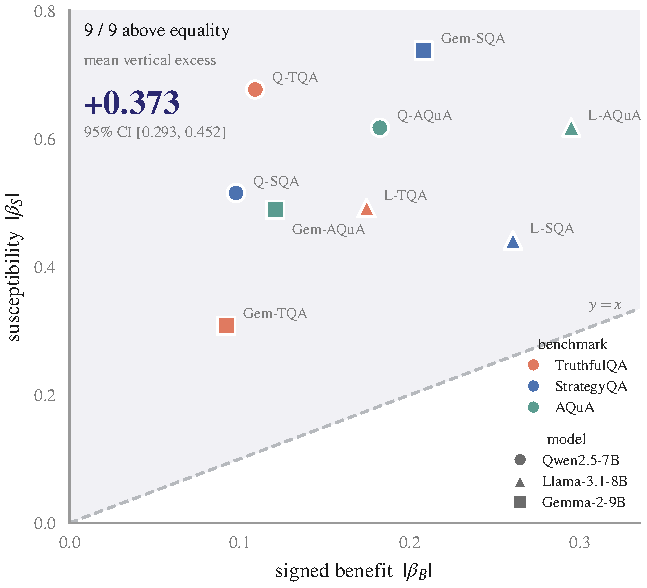
\includegraphics[width=\columnwidth]{figures/f14_smb_pair_slopes.pdf}
\caption{\textbf{Margin tracks susceptibility more strongly than signed benefit in all nine pairs.} Points show absolute slopes, connected within pairs. The equal-pair macro contrast is $+0.373$ ($95\%$ CI $[0.293,0.452]$); per-pair estimates are in Appendix~\ref{sec:app-smb}.}
\label{fig:smb-pairs}
\vspace{-3pt}
\end{figure}

\subsection{A Margin Gate Improves Intervention Targeting}
\label{sec:sgir-main}

The pre-registered gate uses the original margin to choose whether to switch to separately assigned evidence. A seeded, pair-stratified $50/50$ split keeps all eight replicates of each question together. Development selects $7/11$, frozen before the single test evaluation. KEEP retains all original answers; RERUN-ALL switches all; RANDOM matches the gate's intervention count within each pair (Appendix~\ref{sec:app-sgir}).

The gate acts on $675/2880$ test episodes ($23.4\%$), reaching $74.34\%$ accuracy. It beats RANDOM by $1.21$ percentage points ($95\%$ CI $[0.31,2.15]$), KEEP by $1.42$ ($[0.28,2.60]$), and RERUN-ALL by $0.94$ ($[0.07,1.81]$; Table~\ref{tab:sgir-main}). Inference resamples $360$ question clusters.

Among gated episodes, the switch corrects errors in $16.0\%$ and introduces errors in $9.9\%$. Margin thus contains actionable information, but the benefit varies across pairs (Table~\ref{tab:sgir-heterogeneity}). Qwen and Llama improve over KEEP overall; Gemma is flat or negative. Only the Qwen/AQuA and Llama/AQuA gate-minus-RANDOM intervals exclude zero. All aggregate gains remain below the pre-specified $5$-point practical threshold, while the gate uses $76.6\%$ fewer extra calls than RERUN-ALL ($2.58$ per episode).

\begin{table}[t]
\centering\footnotesize
\setlength{\tabcolsep}{4pt}
\renewcommand{\arraystretch}{1.06}
\caption{Test accuracy and paired policy differences: $2880$ episodes in $360$ question clusters, $675$ gated. CIs cluster by question; RANDOM matches budget within each pair.}
\label{tab:sgir-main}
\begin{tabularx}{\columnwidth}{@{}Zrr@{}}
\toprule
Policy & Accuracy & $95\%$ CI\\
\midrule
KEEP & $0.7292$ & $[0.6885, 0.7684]$\\
RERUN-ALL & $0.7340$ & $[0.6903, 0.7764]$\\
RANDOM@budget & $0.7312$ & $[0.6899, 0.7708]$\\
\rowcolor{resultgray}
\resultcell{Margin gate} & \resultcell{$0.7434$} & \resultcell{$[0.7014, 0.7837]$}\\
\midrule
\multicolumn{3}{@{}l}{Paired differences (gate $-$ comparator)}\\
\rowcolor{resultgray}
\resultcell{Gate $-$ RANDOM} & \resultcell{$+0.0121$} & \resultcell{$[+0.0031, +0.0215]$}\\
Gate $-$ KEEP & $+0.0142$ & $[+0.0028, +0.0260]$\\
Gate $-$ RERUN-ALL & $+0.0094$ & $[+0.0007, +0.0181]$\\
\bottomrule
\end{tabularx}
\end{table}

\begin{table}[t]
\centering\footnotesize
\setlength{\tabcolsep}{4pt}
\renewcommand{\arraystretch}{1.02}
\caption{Gate minus RANDOM in percentage points. Bold cells have pointwise $95\%$ CIs excluding zero; intervals are in Appendix~\ref{sec:app-sgir}.}
\label{tab:sgir-heterogeneity}
\begin{tabularx}{\columnwidth}{@{}Zrrr@{}}
\toprule
Model & TruthfulQA & StrategyQA & AQuA\\
\midrule
Qwen & $+1.45$ & $-0.36$ & $\mathbf{+3.57}$\\
Llama & $+1.80$ & $+1.31$ & $\mathbf{+3.97}$\\
Gemma & $+0.04$ & $-1.23$ & $+0.39$\\
\bottomrule
\end{tabularx}
\end{table}

\paragraph{Mechanism-specific repair remains unresolved.}
The pre-registered matched-$G$ recovery comparison detects no population-level difference ($-0.70$ points, $95\%$ CI $[-2.57,1.15]$). All five macro intervals include zero across calipers $0.02/0.05/0.10$, nearest-neighbour matching, and the nested LPM; differing reference arms limit interpretation (Appendix~\ref{sec:app-mmrt}).

\section{Limitations}

\label{sec:limitations}

Agreement matching leaves differences in error correlation, question selection, and reference arms. Copying noise uses a baseline proxy, and corrected directional components assume a noise allocation. Margin regressions are associations; fresh sampling and participation changes can fall outside the theoretical vote-reassignment model. Separately assigned evidence may retain dependence, so its gain need not equal IRIC headroom.

Generalization is limited to six model families, six benchmarks, reused evidence pools, and four evaluation replicates per question. Cluster-resampling checks have six clusters per axis, and accuracy ceilings restrict easy-question effects. The gate covers nine pairs and one margin-only policy, with uneven gains. Mechanism-specific repair requires both interventions to be tested on both mechanism states.

\section{Conclusion}
\label{sec:conclusion}

Dependence alone does not determine collective accuracy or justify reducing it. Equal pairwise correlations can yield different majority accuracies; margins constrain answer changes; independent-reference recovery gains break minus rescue. Empirically, copying changes more answers at matched agreement without a significant average accuracy gap. Margin tracks susceptibility more strongly than benefit, yet a held-out gate beats random intervention at equal budget by $1.21$ points while acting on fewer than a quarter of episodes. The modest, uneven gain shows why interventions should be judged by the errors they correct and introduce.

\clearpage

\bibliography{tacl2021}
\bibliographystyle{acl_natbib}

\clearpage

\appendix

% Appendix layout: keep natural text spacing instead of stretching short columns.
\raggedbottom

% Compact appendix paragraphs and display equations without changing font size.
\setlength{\parskip}{0pt}
\setlength{\smallskipamount}{2pt plus 1pt minus 1pt}
\setlength{\medskipamount}{3pt plus 1pt minus 1pt}
\setlength{\abovedisplayskip}{5pt plus 1pt minus 1pt}
\setlength{\belowdisplayskip}{5pt plus 1pt minus 1pt}
\setlength{\abovedisplayshortskip}{2pt plus 1pt}
\setlength{\belowdisplayshortskip}{4pt plus 1pt minus 1pt}
\setlength{\textfloatsep}{5pt plus 1pt minus 1pt}
\setlength{\floatsep}{3pt plus 1pt minus 1pt}
\setlength{\intextsep}{7pt plus 1pt minus 1pt}
\setlength{\partopsep}{0pt}
\setlength{\aboverulesep}{0.4ex}
\setlength{\belowrulesep}{0.4ex}
\setlength{\dbltextfloatsep}{5pt plus 1pt minus 1pt}
\setlength{\dblfloatsep}{3pt plus 1pt minus 1pt}
\setlength{\abovecaptionskip}{4pt}
\setlength{\belowcaptionskip}{3pt}
\setcounter{topnumber}{4}
\setcounter{totalnumber}{6}
\setcounter{dbltopnumber}{4}
\renewcommand{\topfraction}{0.95}
\renewcommand{\textfraction}{0.05}
\renewcommand{\floatpagefraction}{0.60}
\renewcommand{\dbltopfraction}{0.95}
\renewcommand{\dblfloatpagefraction}{0.60}
% Stack float-only pages tightly from the top.
\makeatletter
\setlength{\@fptop}{0pt}
\setlength{\@fpsep}{3pt}
\setlength{\@fpbot}{0pt plus 1fil}
\setlength{\@dblfptop}{0pt}
\setlength{\@dblfpsep}{3pt}
\setlength{\@dblfpbot}{0pt plus 1fil}
\makeatother


\section{Notation}
\label{sec:notation}

Table~\ref{tab:notation} distinguishes potentially confusable quantities.
Indicators use $\mathbf1[\cdot]$; logarithms are natural.

\begin{table}[!htbp]
\centering\footnotesize
\setlength{\tabcolsep}{3pt}
\renewcommand{\arraystretch}{1.0}
\caption{Selected notation: distinctions used in the analysis.}
\label{tab:notation}
\begin{tabularx}{\columnwidth}{@{}lZ@{}}
\toprule
\textbf{Symbols} & \textbf{Distinction}\\
\midrule
$\Dep, G$ & Error correlation across repeated draws versus vote agreement within a realization.\\
$\rho,\tetra(\rho)$ & Latent Gaussian correlation versus induced binary error correlation.\\
$\chi(m),\eta(m)$ & Probability of sufficient reach versus actual decision change, conditional on margin.\\
$\Hrep,\Delta A$ & Independent-reference recovery $A_0-A_g$ versus intervention effect $A_g-A_0$.\\
$E_i,\widetilde E_{ri}$ & Theoretical error versus frozen score coding, which treats flat responses as correct.\\
$\widehat p_{\mathrm{bin}},A_{\mathrm{none}}$ & Agent-level binning accuracy versus collective no-evidence accuracy.\\
$\widehat{\Marg}_{\mathrm{base}}$ & Margin pooled across no-evidence replicates, distinct from a realized reference margin.\\
$C_{\mathrm{within}},\delta C$ & Within-arm disagreement and descriptive excess change $\delta C=\Delta Y-C_{\mathrm{within}}$.\\
\bottomrule
\end{tabularx}
\end{table}

\section{Problem Formulation}
\label{sec:problem-formulation}

\paragraph{Canonical scores and participation.}

Decisions follow Section~\ref{sec:main-quantities}. Stored truth is $\Truth=0$.
Flat scores and parse failures cast no vote; empirical margins use the retained
count $n_{\mathrm{tot}}=\sum_j n_j$.

\paragraph{Computable dependence.}
For the replicate error matrix $E\in\{0,1\}^{R\times N}$, variance
expansion rewrites Equation~\ref{eq:main-dep} as
\begin{equation}
\Dep(q)=\frac{\mathrm{Var}(\sum_i E_i)-\sum_i\sigma_i^2}
{(\sum_i\sigma_i)^2-\sum_i\sigma_i^2}.
\label{eq:D}
\end{equation}

Covariance requires repeated draws at fixed question and condition. Pooling
and missing-value rules are in Appendix~\ref{sec:app-est-dep}.

\begin{definition}[IRIC intervention]
\label{def:iric}
An independence-restoring, information-conserving intervention draws fresh
votes from the independent baseline law at the same question, preserving
per-agent information distributions and the voting rule. This defines a
reference intervention rather than a query-free implementation.
\end{definition}

\section{Dependence Models and Evidence Assignment}
\label{sec:methodology}

\subsection{Two Mechanisms}
\label{sec:dependence-mechanisms}

\paragraph{Upstream shared evidence.}
A common evidence variable enters each agent's private formation of belief
before any aggregation. In a Gaussian-threshold idealization with marginal
competence $p$, take $0\le\rho\le1$, write $a=\Phi^{-1}(p)$, and set
\begin{equation}
C_i=\mathbf{1}\!\left[\sqrt{\rho}\,Z_0+\sqrt{1-\rho}\,\epsilon_i\le a\right],
\label{eq:m1}
\end{equation}
where $Z_0,\epsilon_1,\ldots,\epsilon_N$ are independent standard normals.
Here $E_i=1-C_i$, so error and correctness correlations coincide.
Each $C_i$ has competence $p$, while its pairwise correlation is
\begin{equation}
\tetra(\rho)=\frac{\Phi_2(a,a;\rho)-p^2}{p(1-p)}.
\label{eq:tau}
\end{equation}
\begin{lemma}[Dependence calibration]
\label{lem:calibration}
For $p\in(0,1)$, $\tetra$ is a strictly increasing bijection of $[0,1]$
onto itself, with $\tetra(\rho)<\rho$ for $0<\rho<1$.
\end{lemma}
Thus measured correlation can calibrate latent $\rho$ in this idealization;
its upstream graph is $Z_0\to C_i\to Y$.

\paragraph{Downstream copying.}

For categorical votes $X^{(t)}=(X_1^{(t)},\ldots,X_N^{(t)})$,
$\Plur(X^{(t)})$ denotes their plurality. The idealized synchronous operator
makes every agent adopt the unique plurality:

\begin{equation}
X_i^{(t+1)}=Y_t=\Plur\!\left(X^{(t)}\right).
\label{eq:m2}
\end{equation}

Uniqueness holds under Theorem~\ref{thm:nonequiv}'s odd binary assumptions.
The feedback graph is $X^{(t)}\to Y_t\to X^{(t+1)}$; empirical graded
copying uses Table~\ref{tab:prompts-peer}.

\subsection{A Matched Evidence-Assignment Design}
\label{sec:matched-instrument}

The evidence design fixes content distribution, framing, question, option
order, population size, and voting rule, varying only assignment:

\begin{description}
\setlength{\itemsep}{0pt}
\setlength{\parsep}{0pt}
  \item[\nocond] no evidence is supplied.
  \item[\shared] one evidence item is drawn and broadcast to all $N$ agents, a
  common shock.
  \item[\indep] agents receive items from a random permutation of the same
  de-duplicated pool, continuing with fresh permutations if the pool is
  smaller than $N$.
\end{description}

This estimates evidence-assignment effects, without randomizing copying
versus sharing or identifying a causal effect of scalar $\Dep$. Each pool
pass samples without replacement; clues repeat only if $|\mathcal U_q|<N$.
Fresh draws per replicate identify

\begin{equation}
\Delta \Dep=\Dep(\shared)-\Dep(\indep)
\label{eq:dD}
\end{equation}

Positive values indicate greater score-coded dependence under common evidence
(Appendix~\ref{sec:app-est-dep}). Algorithm~\ref{alg:instrument} stores canonical
scores with option order fixed across arms and replicates.

\begin{figure}[!htbp]
\small
\setlength{\tabcolsep}{2pt}
\noindent\begin{tabularx}{\columnwidth}{@{}r@{\ \,}Z@{}}

\toprule
\multicolumn{2}{@{}l@{}}{\algname{One matched-instrument cell.}\label{alg:instrument}}\\
\midrule
 & \lvA\algin\ questions $Q$, options per question, agents $1..N$,
   replicates $R$, evidence pool $\mathcal{P}_q$ per question, conditions
   $\{\nocond,\shared,\indep\}$\\
 & \lvA\algout\ score tensor $T[\,c,q,r,i,\cdot\,]$ in canonical
   coordinates\\
\midrule
1 & \lvA\algfor\ $q\in Q$:\\
2 & \lvB $\mathcal{U}_q\leftarrow$ \textsc{dedup}$(\mathcal{P}_q)$\\
3 & \lvB draw a question-fixed permutation $\pi$; displayed position
   $\ell$ contains canonical option $\pi(\ell)$, $\ell=0..K-1$\\
4 & \lvB\algfor\ $r=0..R-1$:\\
5 & \lvC seed a fresh replicate stream $\xi_{q,r}$\\
6 & \lvC\algfor\ $c\in\{\nocond,\shared,\indep\}$:\\
7 & \lvD\algif\ $c=\nocond$: $e_1..e_N\leftarrow\varnothing$\\
8 & \lvD\algelse\ \algif\ $c=\shared$: draw one $u$ uniformly from
   $\mathcal{U}_q$ using $\xi_{q,r}$; $e_1..e_N\leftarrow\textsc{frame}(u)$
   \{common shock\}\\
9 & \lvD\algelse:\\
10 & \lvE take $u_1..u_N$ from random permutations of $\mathcal{U}_q$,
   exhausting each pass before refilling; $e_i\leftarrow\textsc{frame}(u_i)$\\
11 & \lvD $x_i\leftarrow$ \textsc{elicit}$(q,\text{options in order }\pi,e_i)$
   for $i=1..N$, in parallel\\
12 & \lvD $T[c,q,r,i,\pi(\ell)]\leftarrow x_i[\ell]$ for every $i,\ell$
   \{scores restored to canonical indices\}\\
\midrule
 & \lvA\algret\ $T$ for offline estimation
   (Appendix~\ref{sec:app-estimators}).\\
\bottomrule
\end{tabularx}
\end{figure}

Evidence excludes agent answers and peer states; copying uses the separate
peer block in Table~\ref{tab:prompts-peer}.

\section{Scope and Assumptions}
\label{sec:theory}
\label{sec:dependence-measurement}
\label{sec:decision-susceptibility}
\label{sec:repairability-method}
\label{sec:mechanism-non-equivalence}

\subsection{Susceptibility and Regression}
\label{sec:susceptibility-analysis}

Parsing failures and fresh sampling can violate the gate's fixed-participation
reassignment model. Breadth margins pool all eight no-evidence replicates,
including evaluation draws, and are therefore neither realized reference
margins nor sample-disjoint. Matching uses mean independent-evidence margins
for sharing and $g=0$ margins for copying.

For $U=|\Delta A(q)|$, a non-increasing conditional mean
$f(m)=\mathbb E[U\mid\Marg=m]$ and
$0<\mathrm{Var}(\Marg)<\infty$ are sufficient for a non-positive
population regression slope. Individual vote-change bounds do not imply
the conditional binomial domination in Equation~\ref{eq:main-reach-tail}.

\subsection{Repair Headroom and Coupling}
\label{sec:repairability-bounds}

With question, truth, and arm marginals fixed, pairing can change motion,
break, and rescue rates, but preserves break minus rescue. Choosing at the
population level between retention and IRIC gives gain $\max\{0,\Hrep\}$;
this assumes neither question-wise oracle selection nor baseline optimality.

\section{Proofs}
\label{sec:app-proofs}

\paragraph{Calibration (Lemma~\ref{lem:calibration}).}
For $a=\Phi^{-1}(p)$, Mehler's expansion gives
$\tetra(\rho)=\sum_{k\ge1}w_k\rho^k$ with
$w_k=\varphi(a)^2\He_{k-1}(a)^2/[k!p(1-p)]\ge0$ and $w_1>0$.
The endpoint $\tetra(1)=1$ gives $\sum_kw_k=1$ by monotone convergence.
Since $\He_1(a)=a$ and $\He_2(a)=a^2-1$ cannot both vanish, some
$w_k$ with $k>1$ is positive. Therefore $\tetra(\rho)<\rho$ on $(0,1)$;
$\tetra'(\rho)\ge w_1>0$ for $0\le\rho<1$, and continuity at the endpoints
gives the bijection. We use the probabilists' normalization
$\He_k(x)=(-1)^k e^{x^2/2}(d^k/dx^k)e^{-x^2/2}$.
\hfill$\square$

\paragraph{Non-equivalence (Theorem~\ref{thm:nonequiv}).}
As $\rho\to1$, the Gaussian-threshold correctness indicators converge
almost surely to $\mathbf1[Z_0<a]$. Their majority therefore has limiting
accuracy $\Phi(a)=p$. Synchronous copying sets every vote equal to $Y_0$
and preserves that answer thereafter. Both terminal error vectors have
identical nonconstant entries, so their dependence is one. For odd
$N=2\ell+1$, the binomial recursion gives
\begin{equation*}
\begin{split}
P_{\mathrm{maj}}(N,p)-p
={}&(2p-1)\\
&\cdot\sum_{j=1}^{\ell}\binom{2j-1}{j-1}[p(1-p)]^j,
\end{split}
\end{equation*}
which has the sign of $p-1/2$. \hfill$\square$

\paragraph{Insufficiency (Proposition~\ref{cor:insufficient}).}
For $N=3$, let $J$ count correct votes and choose the correct subset
uniformly given $J$. Take
$\Pr(J=0,1,2,3)=(8,36,54,27)/125$ or $(7,39,51,28)/125$.
Both laws have $\mathbb E[J]/3=3/5$ and
$\mathbb E[J(J-1)]/6=9/25$, giving the same marginals and pairwise
correctness, hence error, correlations zero. However,
$\Pr(J\ge2)=81/125$ or $79/125$. \hfill$\square$

\paragraph{Sharp gate (Lemma~\ref{lem:gate}).}
Each reassigned vote reduces a leader--competitor gap by at most two, so
a positive gap $d-2\kappa$ protects the winner. Transferring
$\lceil d/2\rceil$ leader votes to the runner-up is feasible and makes
that competitor tie or overtake the original leader, attaining the lower
bound on reach. \hfill$\square$

\paragraph{Susceptibility (Theorem~\ref{thm:gating}).}
Pointwise,
$|\mathcal A_g-\mathcal A_0|\le\mathbf1[Y_g\neq Y_0]
\le\mathbf1[\kappa\ge\lceil N\Marg/2\rceil]$.
Conditional expectation and the triangle inequality give
Equation~\ref{eq:gating-bound}; averaging gives the unconditional bound.
Conditional binomial domination and the Chernoff upper-tail bound give
Equation~\ref{eq:main-reach-tail} only when $m/2>s$.
For the separate regression claim, an independent copy $\Marg'$ yields
\begin{equation*}
\begin{split}
2\mathrm{Cov}(\Marg,f(\Marg))
={}&\mathbb E\big[(\Marg-\Marg')\\
&\cdot(f(\Marg)-f(\Marg'))\big]\le0
\end{split}
\end{equation*}
when $f$ is non-increasing. \hfill$\square$

\paragraph{Partition and headroom (Proposition~\ref{prop:identity}; Theorem~\ref{thm:headroom}).}
Classifying a changed decision by initial and final correctness gives the
disjoint events $B,S,C$. Moreover,
$\mathcal A_0-\mathcal A_g=\mathbf1[B]-\mathbf1[S]$ pointwise.
Taking expectations proves Equation~\ref{eq:main-identity}. IRIC restores
the law of $Y_0$, so $A_{\mathcal R}=A_0$. The triangle inequality gives
$|\pbreak-\prescue|\le\pbreak+\prescue=\Delta Y-\pchurn$;
subtracting signed headroom from motion gives $2\prescue+\pchurn$.
Nonnegativity gives the stated equality conditions. \hfill$\square$

\section{Prompts}
\label{sec:app-prompts}
\label{sec:app-prompts-evidence}
\label{sec:app-prompts-copying}

Table~\ref{tab:prompts-elicit} reproduces primary directives and the generator verbatim, with normalized line breaks; weak framing and fallback are summarized. Braces mark substitutions. Evidence and peer wrappers begin with ``Reference information or evidence for this question:'' and ``Current views of the other agents in the group:''; absent blocks are empty. Soft copying is outside $g\in\{0,1,2\}$; \texttt{\{pct\}} is $\mathrm{round}(100g)$ and \texttt{\{distribution\}} lists up to three peer counts.

Clues exclude peer choices and are deduplicated. Parsing accepts labels, text, or indices, scores omitted options below the minimum, and retries flat replies twice before omitting their votes.

\section{Collection Protocol}
\label{sec:app-protocol}

\paragraph{Model settings and option order.}

Settings follow Section~\ref{sec:experimental-setup}. Evaluation fixes
within-cell option order across arms and replicates; truth is stored as $0$.

\subsection{The Condition Grid}
\label{sec:app-conditions}

Seven conditions cover baseline, shared evidence (correct/misleading
$\times$ weak/strong framing), and separately assigned evidence
(correct/misleading, strong framing). Breadth uses baseline and both
correct/strong arms. Clues are redrawn per replicate by the pool-pass rule
(Appendix~\ref{sec:matched-instrument}); control-arm dependence may persist.

\subsection{Competence Strata by Split Sample}
\label{sec:app-strata}

Probe/evaluation shuffling uses dataset indices/subset positions. Different
option orders can invalidate probe difficulty labels; within-cell contrasts
remain matched. Breadth pools both original sets, bins on baseline replicates
$0$--$3$, and evaluates on $4$--$7$ with the main-text support rules.
Mechanism matching uses both sets and all eight replicates without rebinning.

\paragraph{Reproducibility.}
\label{sec:app-repro}
Score tensors and caches retain condition/question/replicate/agent indices,
models, input hashes, option displays, evidence, and responses, enabling
prompt reconstruction and reanalysis without new model calls.

\section{Estimators and Statistical Procedures}
\label{sec:app-estimators}

\subsection{Dependence}
\label{sec:app-est-dep}

Matching uses $G$ (legacy field \texttt{D}). Breadth uses
$\widetilde E_{ri}=\mathbf1[\arg\max_j T[c,q,r,i,j]\neq0]$ and pools
question numerators and denominators before division. Saturated questions
contribute zero to both, avoiding error-variance selection. The released
estimate is \texttt{dD\_pooled}, replacing the mean of question ratios.
For flat scores, arg-max returns truth index $0$, so the frozen estimator
codes $\widetilde E=0$; binning counts flats as incorrect among $4N$ attempts,
and voting omits them. Theoretical error coding therefore agrees only for
informative responses. Recoding flats as errors preserves all $66$ signs
($63$ positive); null calibration retains frozen coding.

\subsection{Decision Change and Ties}
\label{sec:app-est-dy}

Answer-change rates pair replicate indices and satisfy
Equation~\ref{eq:main-identity} question-wise. Matching treats ties as
non-answers; equivalence uses seeded tie breaking. Both give positive macro
excess intervals (Table~\ref{tab:churn-results}). $C_{\mathrm{within}}$ averages
both arms' disagreement over unordered held-out replicate pairs. Subtraction
gives descriptive excess motion, rather than noise-free directional rates.

\subsection{Agreement-Matched Mechanism Comparison}
\label{sec:app-est-matched}

Caliper matching averages shared outcomes within
$\varepsilon\in\{0.02,0.05,0.10\}$ of each copying observation's $G$.
Intervals require five matches; bootstraps resample complete matches within
pairs, then whole pairs for macro estimates. Coverage is in
Table~\ref{tab:matched-pair-results}. Nested LPMs add mechanism and its $G$
interaction, assessed by $F$-tests. Nearest-neighbour matching standardizes
$G$, reference accuracy, and margin (Figure~\ref{fig:robustness}).

\subsection{Accuracy Effects by Difficulty}
\label{sec:app-est-regime-battery}

The pre-specified H1--H4 analyses cover $66$ strata.
H1 compares the sign of $\Delta A$ with
$\mathrm{sign}(A_{\mathrm{none}}-P_{\mathrm{maj}}(11,A_{\mathrm{none}}))$;
H4 correlates this proxy with $\Delta A$
(diagnostics below). Here $A_{\mathrm{none}}$
is collective no-evidence accuracy, not agent competence
$\widehat p_{\mathrm{bin}}$, so these are not direct tests of
Theorem~\ref{thm:nonequiv}.

H2 uses the $\pm0.05$ equivalence margin fixed before sweep completion;
regime estimates are primary (Table~\ref{tab:accuracy-results}).
The pooled descriptive mean is $-0.0092$ ($95\%$ CI
$[-0.0182,-0.0008]$; $90\%$ CI $[-0.0168,-0.0020]$).
H3's easy-minus-hard effect across $30$ paired model--benchmark units is
$0.0013$ ($95\%$ CI $[-0.0190,0.0210]$).

\paragraph{Additional diagnostics.}
\label{sec:app-additional-diagnostics}
Easy-question excess change is $0.43$ points ($95\%$ CI $[0.10,0.87]$); hard-question excess is $5.2\%$ of raw changes. Tie-rule, weighting, and benchmark-resampling checks remain positive; model resampling crosses zero on hard questions (Table~\ref{tab:churn-results}). Excess variability does not identify a noise-free effect.

The proxy matches $12/28$ signs ($p=0.83$; $r=-0.18$, $95\%$ CI $[-0.44,0.05]$). Baseline margins track smaller absolute hard-question effects (slope $-0.063$, CI $[-0.112,-0.012]$), beyond what the theorem implies. Joint ceilings constrain $15/31$ easy strata (Figure~\ref{fig:susceptibility}).

\subsection{Intervals and Units of Replication}
\label{sec:app-est-ci}

Percentile CIs use $95\%$ confidence ($90\%$ for equivalence), resampling
questions within cells, breadth strata, or nine mechanism pairs as appropriate.
Model/benchmark sensitivity CIs use six clusters per axis and are approximate.
Matching support and precision are reported in
Table~\ref{tab:matched-coverage} and Figure~\ref{fig:estimability}.

\FloatBarrier
\section{Supplementary Result Tables}
\label{sec:app-result-tables}

The tables distinguish primary estimates from sensitivity analyses.
Independent rounding can shift component sums by $0.0001$.

\subsection{Dependence, Decision Motion, and Accuracy}
\label{sec:app-tab-breadth}

\begin{table}[H]
\centering\footnotesize
\setlength{\tabcolsep}{3pt}
\renewcommand{\arraystretch}{1.06}
\caption{Breadth effects (fractions) and sensitivity. Answer changes use non-answer ties unless marked seeded; accuracy uses seeded tie breaking.}
\label{tab:churn-results}
\label{tab:accuracy-results}
\label{tab:tie-sensitivity}
\begin{tabularx}{\columnwidth}{@{}Zrr@{}}
\toprule
Quantity & Hard & Easy\\
\midrule
Strata & 35 & 31\\
Raw $\Delta Y$ & $0.2704$ & $0.0187$\\
$C_{\mathrm{within}}$ & $0.2563$ & $0.0144$\\
\rowcolor{resultgray}
\resultcell{Excess $\delta C$} & \resultcell{$0.0140$} & \resultcell{$0.0043$}\\
\rowcolor{resultgray}
\resultcell{Stratum $95\%$ CI} & \resultcell{$[0.0019, 0.0247]$} & \resultcell{$[0.0010, 0.0087]$}\\
Model-cluster $95\%$ CI & $[-0.0041, 0.0294]$ & $[0.0006, 0.0077]$\\
Benchmark-cluster $95\%$ CI & $[0.0061, 0.0226]$ & $[0.0004, 0.0100]$\\
\midrule
Raw $\Delta Y$ (seeded) & $0.2447$ & $0.0182$\\
Excess $\delta C$ (seeded) & $0.0119$ & $0.0046$\\
$95\%$ CI (seeded) & $[0.0004, 0.0221]$ & $[0.0010, 0.0090]$\\
\midrule
\rowcolor{resultgray}
\resultcell{Mean $\Delta A$} & \resultcell{$-0.0095$} & \resultcell{$-0.0089$}\\
\rowcolor{resultgray}
\resultcell{\mbox{$90\%$ CI for $\Delta A$}} & \resultcell{$[-0.0214, 0.0020]$} & \resultcell{$[-0.0172, -0.0015]$}\\
\bottomrule
\end{tabularx}
\par\smallskip
\begin{minipage}{\columnwidth}\footnotesize
Accuracy CIs lie within $\pm0.05$. Six-cluster percentile CIs are approximate. Shading marks primary estimates; other intervals assess sensitivity.
\end{minipage}
\end{table}

\begin{table}[H]
\centering\small
\setlength{\tabcolsep}{3pt}
\caption{Positive dependence signs: two marginal breakdowns of the same 66 strata.}
\label{tab:instrument-results}
\begin{tabularx}{\columnwidth}{@{}Zrr@{}}
\toprule
Model / benchmark & Positive/usable & Fraction\\
\midrule
Qwen2.5-7B & 11/12 & 91.7\%\\
Llama-3.1-8B & 10/10 & 100.0\%\\
Gemma-2-9B & 10/11 & 90.9\%\\
Mistral-7B & 11/11 & 100.0\%\\
Phi-4-mini & 10/10 & 100.0\%\\
DeepSeek-R1-7B & 11/12 & 91.7\%\\
\midrule
TruthfulQA & 9/11 & 81.8\%\\
AQuA & 9/9 & 100.0\%\\
ARC-Challenge & 11/12 & 91.7\%\\
CommonsenseQA & 12/12 & 100.0\%\\
MMLU & 10/10 & 100.0\%\\
StrategyQA & 12/12 & 100.0\%\\
\midrule
\rowcolor{resultgray}
\resultcell{Overall} & \resultcell{63/66} & \resultcell{95.5\%}\\
\bottomrule
\end{tabularx}
\par\smallskip
\begin{minipage}{\columnwidth}\footnotesize
Null: $2000$ draws, mean $13.38$, SD $2.79$; $p_{\mathrm{val}}=1/2001\le0.0005$. Six strata lack question support.
\end{minipage}
\end{table}


\par\addvspace{1pt}


\subsection{Agreement-Matched Estimates}
\label{sec:app-tab-mechanism}

\begin{table}[H]
\centering\footnotesize
\setlength{\tabcolsep}{3pt}
\renewcommand{\arraystretch}{1.06}
\caption{Noise corrections for the three mechanism estimators. Copying uses baseline noise as a proxy; single-arm CIs are unavailable.}
\label{tab:mechanism-correction}
\textbf{(a) Single-arm corrections}\par\smallskip
\begin{tabularx}{\columnwidth}{@{}Zrr@{}}
\toprule
Estimator & Shared only & Copy only\\
\midrule
Caliper ($\varepsilon=0.05$) & $0.1633$ & $0.0147$\\
NN-ATT & $0.1964$ & $-0.0625$\\
Nested LPM & $0.2124$ & $0.0101$\\
\bottomrule
\end{tabularx}
\par\smallskip
\textbf{(b) Both-arm correction}\par\smallskip
\begin{tabularx}{\columnwidth}{@{}Zrr@{}}
\toprule
Estimator & Gap & $95\%$ CI\\
\midrule
\rowcolor{resultgray}
\resultcell{Caliper ($\varepsilon=0.05$)} & \resultcell{$0.0595$} & \resultcell{$[0.0315,0.0890]$}\\
NN-ATT & $0.0926$ & $[0.0544,0.1306]$\\
Nested LPM & $0.1086$ & $[0.0772,0.1425]$\\
\bottomrule
\end{tabularx}
\end{table}

% Keep the pair estimates and coverage in separate blocks for column placement.
\begin{table}[H]
\centering\scriptsize
\setlength{\tabcolsep}{3pt}
\renewcommand{\arraystretch}{1.0}
\caption{Copying-minus-shared gaps at caliper $0.05$, pooling regimes within pairs. Estimates have marginal $95\%$ CIs below; coverage is in Table~\ref{tab:matched-coverage}.}
\label{tab:matched-pair-results}
\begin{tabularx}{\columnwidth}{@{}Zrr@{}}
\toprule
Pair & Answer change & Accuracy\\
\midrule
Qwen/TruthfulQA & \shortstack[r]{$0.1060$\\$[0.0479, 0.1666]$} & \shortstack[r]{$0.0559$\\$[0.0222, 0.1000]$}\\
Qwen/StrategyQA & \shortstack[r]{$0.0758$\\$[0.0278, 0.1275]$} & \shortstack[r]{$0.0029$\\$[-0.0531, 0.0509]$}\\
Qwen/AQuA & \shortstack[r]{$0.1515$\\$[0.0920, 0.2127]$} & \shortstack[r]{$-0.0311$\\$[-0.0719, 0.0061]$}\\
Llama/TruthfulQA & \shortstack[r]{$0.2056$\\$[0.1399, 0.2690]$} & \shortstack[r]{$0.0155$\\$[-0.0416, 0.0739]$}\\
Llama/StrategyQA & \shortstack[r]{$0.0806$\\$[0.0303, 0.1354]$} & \shortstack[r]{$-0.0383$\\$[-0.0949, 0.0146]$}\\
Llama/AQuA & \shortstack[r]{$0.2908$\\$[0.2175, 0.3670]$} & \shortstack[r]{$0.0424$\\$[-0.0249, 0.1083]$}\\
Gemma/TruthfulQA & \shortstack[r]{$0.0638$\\$[0.0155, 0.1143]$} & \shortstack[r]{$0.0009$\\$[-0.0381, 0.0401]$}\\
Gemma/StrategyQA & \shortstack[r]{$0.0171$\\$[-0.0132, 0.0558]$} & \shortstack[r]{$0.0061$\\$[-0.0316, 0.0439]$}\\
Gemma/AQuA & \shortstack[r]{$0.0751$\\$[0.0163, 0.1361]$} & \shortstack[r]{$0.0088$\\$[-0.0326, 0.0504]$}\\
\bottomrule
\end{tabularx}
\par\smallskip
\end{table}

\begin{table}[H]
\centering\scriptsize
\setlength{\tabcolsep}{3pt}
\renewcommand{\arraystretch}{1.0}
\caption{Copying-observation match coverage; unlisted pairs have $100\%$ coverage at every caliper.}
\label{tab:matched-coverage}
\begin{tabularx}{\columnwidth}{@{}Zrrr@{}}
\toprule
Pair & $\varepsilon=.02$ & $.05$ & $.10$\\
\midrule
Qwen/TruthfulQA & 97.7\% & 100.0\% & 100.0\%\\
Qwen/StrategyQA & 97.7\% & 97.7\% & 97.7\%\\
Llama/StrategyQA & 96.7\% & 96.7\% & 100.0\%\\
Llama/AQuA & 30.3\% & 100.0\% & 100.0\%\\
Gemma/StrategyQA & 98.1\% & 98.1\% & 98.1\%\\
\bottomrule
\end{tabularx}
\par\smallskip
\raggedright Coverage is the fraction of copying observations with a match.
\end{table}


% Supplementary tables retain the two-column layout.

\subsection{Clustering, Weighting, and Susceptibility}
\label{sec:app-tab-robustness}

\par\addvspace{1pt}
\begin{table}[H]
\centering
\footnotesize
\setlength{\tabcolsep}{2pt}
\renewcommand{\arraystretch}{1.1}
\caption{Copying-minus-shared gaps: (a) primary-caliper components and churn share; (b) raw caliper sensitivity, pair-bootstrap $95\%$ CIs.}
\label{tab:component-results}
\label{tab:caliper-results}
\textbf{(a) Component gaps}\par\smallskip
\begin{tabularx}{\columnwidth}{@{}Zrrrr@{}}
\toprule
Gap & Raw & Shared & Copy & Both\\
\midrule
Motion & $0.1185$ & $0.1633$ & $0.0147$ & $0.0595$\\
Break & $0.0256$ & $0.0439$ & $-0.0006$ & $0.0177$\\
Rescue & $0.0326$ & $0.0509$ & $0.0064$ & $0.0247$\\
Churn & $0.0603$ & $0.0685$ & $0.0088$ & $0.0171$\\
Churn share & $50.9\%$ & $42.0\%$ & $60.1\%$ & $28.8\%$\\
\bottomrule
\end{tabularx}

\par\smallskip
\textbf{(b) Caliper sensitivity}\par\smallskip
\begin{tabularx}{\columnwidth}{@{}Zrrr@{}}
\toprule
$\varepsilon$ & Pairs & Motion gap & $95\%$ CI \\
\midrule
$0.02$ & 9 & $0.1232$ & $[0.0770, 0.1764]$ \\
\rowcolor{resultgray}
\resultcell{$0.05$} & \resultcell{9} & \resultcell{$0.1185$} & \resultcell{$[0.0716, 0.1724]$}\\
$0.10$ & 9 & $0.1118$ & $[0.0623, 0.1674]$ \\
\bottomrule
\end{tabularx}
\par\smallskip
\begin{minipage}{\columnwidth}
\footnotesize (a) Columns name corrected arms. Directional noise allocation is assumed; copying uses baseline noise. Shares use unrounded values. (b) Coverage: Table~\ref{tab:matched-pair-results}.
\end{minipage}
\end{table}

\begin{table}[H]
\centering\footnotesize
\setlength{\tabcolsep}{3pt}
\renewcommand{\arraystretch}{1.06}
\caption{Weighting and margin slopes: $35/31$ hard/easy strata, $1116/1051$ questions. Cluster sensitivity: Table~\ref{tab:churn-results}.}
\label{tab:cluster-results}
\label{tab:weighting-results}
\label{tab:susceptibility-results}
\label{tab:cluster-weighting-results}
\textbf{(a) Question-count weighting}\par\smallskip
\begin{tabularx}{\columnwidth}{@{}Zlrr@{}}
\toprule
Regime & Tie rule & Weighted $\delta C$ & $95\%$ CI\\
\midrule
Hard & Strict & $0.0175$ & $[0.0054, 0.0285]$\\
Easy & Strict & $0.0034$ & $[0.0005, 0.0071]$\\
Hard & Seeded & $0.0143$ & $[0.0025, 0.0251]$\\
Easy & Seeded & $0.0036$ & $[0.0007, 0.0074]$\\
\bottomrule
\end{tabularx}
\par\smallskip
\textbf{(b) Margin slopes}\par\smallskip
\begin{tabularx}{\columnwidth}{@{}Zrr@{}}
\toprule
Diagnostic & Hard & Easy\\
\midrule
Strata & 35 & 31\\
\rowcolor{resultgray}
\resultcell{Mean slope} & \resultcell{$-0.0627$} & \resultcell{$-0.1371$}\\
\rowcolor{resultgray}
\resultcell{$95\%$ CI} & \resultcell{\shortstack[r]{$[-0.1119,$\\$-0.0123]$}} & \resultcell{\shortstack[r]{$[-0.2427,$\\$-0.0500]$}}\\
Zero slopes & 0 & 17\\
Bootstrap significant & 5 & 1\\
Permutation significant & 4 & 6\\
Overlap & 3 & 1\\
\bottomrule
\end{tabularx}
\par\smallskip
\begin{minipage}{\columnwidth}\footnotesize
(a) Equal-stratum estimates: Table~\ref{tab:churn-results}; weighted CIs use the sensitivity run. (b) Significance counts do not test the macro effect; zero slopes need not indicate ceilings.
\end{minipage}
\end{table}
\par\addvspace{1pt}

\subsection{Susceptibility and Signed Benefit}
\label{sec:app-smb}

The pre-registered comparison fits ordinary least squares within each pair
on all $5760$ episodes (Appendix~\ref{sec:app-sgir}), relating KEEP's margin to
\begin{align*}
S&=\mathbf1[Y_{\mathrm{KEEP}}\neq Y_{\mathrm{INDEP}}],\\
B&=\mathbf1[Y_{\mathrm{INDEP}}=\Truth]
 -\mathbf1[Y_{\mathrm{KEEP}}=\Truth].
\end{align*}
The pre-specified contrast $|\beta_S|-|\beta_B|$ pairs slopes from the same
eligible episodes, weights pairs equally, and bootstraps whole pairs
$20{,}000$ times. No policy is selected or pairwise hypothesis tested; these associations
do not estimate $\chi$ or exact IRIC headroom.

\begin{table}[H]
\centering\footnotesize
\setlength{\tabcolsep}{3pt}
\renewcommand{\arraystretch}{1.05}
\caption{Pairwise margin slopes; $640$ eligible episodes per pair except Gemma/AQuA ($638$).}
\label{tab:smb-breakdown}
\begin{tabularx}{\columnwidth}{@{}Zrrr@{}}
\toprule
Pair & $\beta_S$ & $\beta_B$ & $|\beta_S/\beta_B|$\\
\midrule
Qwen/TruthfulQA & $-0.677$ & $-0.109$ & $6.2\times$\\
Qwen/StrategyQA & $-0.515$ & $-0.098$ & $5.3\times$\\
Qwen/AQuA & $-0.617$ & $-0.183$ & $3.4\times$\\
Llama/TruthfulQA & $-0.492$ & $-0.175$ & $2.8\times$\\
Llama/StrategyQA & $-0.441$ & $-0.261$ & $1.7\times$\\
Llama/AQuA & $-0.618$ & $-0.295$ & $2.1\times$\\
Gemma/TruthfulQA & $-0.308$ & $-0.092$ & $3.3\times$\\
Gemma/StrategyQA & $-0.737$ & $-0.208$ & $3.5\times$\\
Gemma/AQuA & $-0.489$ & $-0.121$ & $4.0\times$\\
\bottomrule
\end{tabularx}
\end{table}

\subsection{Confirmatory Margin-Gated Intervention}
\label{sec:app-sgir}

\paragraph{Population and split.}
The nine-pair population and KEEP/INDEP arms follow Section~\ref{sec:experimental-setup}. A seeded, pair-stratified permutation splits $720$ question clusters equally into development/test ($360$ clusters, $2880$ episodes each), hashed and frozen before reading outcomes or margins. Undefined KEEP margins retain the answer.

\paragraph{Threshold selection.}
The gate reads KEEP's margin without extra calls or truth labels. The $N=11$ grid $\{d/m:1\le m\le11,\ 0\le d\le m\}$ has $43$ thresholds. Development selects the largest gain over expected RANDOM accuracy, matching intervention counts within every pair. Ties favor fewer interventions, then smaller thresholds. The selected $\hat\tau=7/11\approx0.636$ is frozen before testing.

\paragraph{Inference.}
One test evaluation uses $20{,}000$ question-cluster bootstrap draws, each with fresh pair-matched RANDOM selection. Shared resamples give paired contrast intervals, which can exclude zero despite overlapping marginal accuracy intervals (Table~\ref{tab:sgir-main}).

\begin{table}[H]
\centering\footnotesize
\setlength{\tabcolsep}{3pt}
\renewcommand{\arraystretch}{1.04}
\caption{Gate intervention and conditional harmful/helpful rates by pair ($320$ test episodes each). Accuracy gains are in Table~\ref{tab:sgir-pair-gains}.}
\label{tab:sgir-breakdown}
\begin{tabularx}{\columnwidth}{@{}Zrrr@{}}
\toprule
Pair & Gated & Harmful & Helpful\\
\midrule
Qwen/TruthfulQA & $16.2\%$ & $0.077$ & $0.192$\\
Qwen/StrategyQA & $13.8\%$ & $0.227$ & $0.182$\\
Qwen/AQuA & $40.9\%$ & $0.076$ & $0.183$\\
Llama/TruthfulQA & $23.8\%$ & $0.092$ & $0.184$\\
Llama/StrategyQA & $19.4\%$ & $0.065$ & $0.161$\\
Llama/AQuA & $57.8\%$ & $0.086$ & $0.173$\\
Gemma/TruthfulQA & $5.6\%$ & $0.000$ & $0.000$\\
Gemma/StrategyQA & $1.9\%$ & $0.667$ & $0.000$\\
Gemma/AQuA & $31.8\%$ & $0.119$ & $0.099$\\
\bottomrule
\end{tabularx}
\par\smallskip
\end{table}

\begin{table}[H]
\centering\footnotesize
\setlength{\tabcolsep}{3pt}
\renewcommand{\arraystretch}{1.04}
\caption{Gate-minus-RANDOM accuracy gains with pointwise $95\%$ CIs; shaded intervals exclude zero. Each pair has $320$ test episodes.}
\label{tab:sgir-pair-gains}
\begin{tabularx}{\columnwidth}{@{}Zrr@{}}
\toprule
Pair & Gain & $95\%$ CI\\
\midrule
Qwen/TruthfulQA & $+0.0145$ & $[-0.0031,0.0375]$\\
Qwen/StrategyQA & $-0.0036$ & $[-0.0344,0.0281]$\\
\rowcolor{resultgray}
\resultcell{Qwen/AQuA} & \resultcell{$+0.0357$} & \resultcell{$[0.0031,0.0719]$}\\
Llama/TruthfulQA & $+0.0180$ & $[-0.0125,0.0531]$\\
Llama/StrategyQA & $+0.0131$ & $[-0.0063,0.0375]$\\
\rowcolor{resultgray}
\resultcell{Llama/AQuA} & \resultcell{$+0.0397$} & \resultcell{$[0.0031,0.0750]$}\\
Gemma/TruthfulQA & $+0.0004$ & $[0.0000,0.0031]$\\
Gemma/StrategyQA & $-0.0123$ & $[-0.0344,0.0000]$\\
Gemma/AQuA & $+0.0039$ & $[-0.0281,0.0344]$\\
\bottomrule
\end{tabularx}
\end{table}

Of net recovery over KEEP, Llama contributes $71\%$, Qwen $44\%$, and Gemma $-15\%$. Gemma/StrategyQA gates only six episodes, making its conditional rates imprecise. Aggregate recovery and cost are in Section~\ref{sec:sgir-main}.

\subsection{Reference-Arm Recovery at Matched Agreement}
\label{sec:app-mmrt}

This pre-registered secondary analysis reuses the nine-pair rows and estimators with recovery gain (reference minus mechanism-state accuracy) as outcome. References are separately assigned evidence for sharing and final $g=0$ for copying; neither guarantees IRIC. Matching uses $G$ (legacy field \texttt{D}), with primary caliper $0.05$ and sensitivities $0.02/0.10$. Macro estimates weight pairs equally and bootstrap pairs $20{,}000$ times.

Table~\ref{tab:mmrt-breakdown} summarizes all five comparisons. Primary-caliper coverage is at least $96.7\%$ in every pair. Qwen/TruthfulQA alone has intervals excluding zero at all three calipers (primary gap $-5.59$ points, $95\%$ CI $[-9.59,-2.00]$), a descriptive result. Mechanism-specific repair requires both interventions on both states; existing enrichment actions cover only copying.

\begin{table}[H]
\centering\footnotesize
\setlength{\tabcolsep}{3pt}
\renewcommand{\arraystretch}{1.02}
\caption{Macro copying-minus-shared recovery gaps (percentage points). All five pre-registered intervals include zero; pairs receive equal weight.}
\label{tab:mmrt-breakdown}
\begin{tabularx}{\columnwidth}{@{}Zrr@{}}
\toprule
Estimator & Gap (pp) & $95\%$ CI\\
\midrule
\rowcolor{resultgray}
\resultcell{Caliper $0.05$} & \resultcell{$-0.70$} & \resultcell{$[-2.57,1.15]$}\\
Caliper $0.02$ & $-1.01$ & $[-4.13,1.66]$\\
Caliper $0.10$ & $-1.20$ & $[-3.03,0.58]$\\
Nearest neighbour & $-0.01$ & $[-2.62,2.81]$\\
Nested LPM & $-1.98$ & $[-5.51,1.20]$\\
\bottomrule
\end{tabularx}
\end{table}


\onecolumn
\section{Supplementary Figures}
\label{sec:app-supplementary-figures}
\label{sec:app-fig-susceptibility}
\label{sec:app-fig-easy-hard}
\label{sec:app-fig-estimability}

\par\addvspace{1pt}

\noindent\begin{minipage}{\textwidth}
\centering
\includegraphics[width=\textwidth]{figures/f6_main_noise_canyon.pdf}
\captionof{figure}{\textbf{Most raw answer changes are close to replicate variability.} \textbf{(a)}, \textbf{(b)} Raw, within-arm, and excess rates by hard/easy stratum; bold lines give means. Lines connect measurements, not time. \textbf{(c)} Excess-change empirical CDFs and rugs. \textbf{(d)} Raw versus corrected ranks, averaging ties.}
\label{fig:noise-canyon}
\end{minipage}
\par\addvspace{6pt}

\noindent\begin{minipage}{\textwidth}
\centering
\includegraphics[width=\textwidth]{figures/f7_main_generalization.pdf}
\captionof{figure}{\textbf{Excess answer changes vary across hard-question cells.} \textbf{(a)} Excess change and \textbf{(b)} accuracy effects by model and benchmark; blanks lack support. \textbf{(c)}, \textbf{(d)} Model and benchmark means. The overall estimate is sensitive to model resampling.}
\label{fig:generalization}
\end{minipage}

\par\addvspace{6pt}

\noindent\begin{minipage}{\textwidth}
\centering
\includegraphics[width=\textwidth]{figures/f9_main_susceptibility.pdf}
\captionof{figure}{\textbf{Margin associations vary with difficulty and group size.} \textbf{(a)} Regime slopes ($15/31$ easy strata at joint ceilings). \textbf{(b)} Model ceiling fractions ($0/5$ to $5/6$). \textbf{(c)} Qwen with $N=5,11,21$: slopes are non-monotonic, most negative at $11$. Test overlap: Figure~\ref{fig:easy-hard}(d).}
\label{fig:susceptibility}
\end{minipage}

\par\addvspace{6pt}

\noindent\begin{minipage}{\textwidth}
\centering
\includegraphics[width=\textwidth]{figures/f10_main_anatomy.pdf}
\captionof{figure}{\textbf{Break, rescue, and churn separate accuracy from answer change.} \textbf{(a)}, \textbf{(b)} Model-wise break/rescue rates on hard/easy questions; diamonds give net effects. \textbf{(c)} Matched pairwise component gaps. \textbf{(d)} Shares of the raw gap. Breadth and matched comparisons differ; raw rates do not establish noise-corrected cancellation.}
\label{fig:anatomy}
\end{minipage}
\par\addvspace{6pt}

\noindent\begin{minipage}{\textwidth}
\centering
\includegraphics[width=\textwidth]{figures/f11-appendix_easy_hard.pdf}
\captionof{figure}{\textbf{Easy-question ceilings limit improvement.} \textbf{(a)}, \textbf{(b)} Shared versus independent accuracy with marginal intervals and equality lines. \textbf{(c)} Easy-stratum accuracy: purple marks joint ceilings; dashes mark missing strata. \textbf{(d)} Significant slope overlap across bootstrap/permutation tests; square area gives stratum fraction.}
\label{fig:easy-hard}
\end{minipage}
\par\addvspace{6pt}

\noindent\begin{minipage}{\textwidth}
\centering
\includegraphics[width=\textwidth]{figures/f12_appendix_estimability.pdf}
\captionof{figure}{\textbf{Estimation support.} \textbf{(a)} Question counts. \textbf{(b)} Excess-change CI width versus support; size indicates noise. \textbf{(c)} Sign-test error rates. \textbf{(d)} Match coverage by caliper.}
\label{fig:estimability}
\end{minipage}
\par\addvspace{6pt}


% Prompt template follows the supplementary diagnostic figures.
\noindent\begin{minipage}{\textwidth}
\centering
\footnotesize
\setlength{\tabcolsep}{3pt}
\renewcommand{\arraystretch}{1.0}
\captionof{table}{Elicitation template and evidence/peer slots (JSON responses). Evidence arms differ only in clue assignment. Peer directives define $g$; $\{c\}/\{m\}$ is the informative-peer top-option fraction. The primary grid uses $g=0,1,2$; Equation~\ref{eq:m2} is idealized.}
\label{tab:prompts-elicit}
\label{tab:prompts-peer}
\begin{tabularx}{\textwidth}{@{}p{0.10\textwidth}p{0.13\textwidth}>{\raggedright\arraybackslash}X@{}}
\toprule
\textbf{Slot} & \textbf{When used} & \textbf{Text} \\
\midrule
\multicolumn{3}{@{}p{\textwidth}@{}}{\emph{Elicitation skeleton. The only prompt that obtains an answer.}}\\
skeleton &
every condition, every $g$ &
\ttfamily\footnotesize \{persona\} Question: \{question\} Options: \{options\} \{evidence\_block\} \{peer\_block\} Think briefly, then rate how strongly you believe EACH label (\{labels\}) is correct, on a scale from -10 to 10, where 10 means certainly correct. Reply with JSON ONLY, in the form \{"scores": \{"A": \textless{}number\textgreater{}, "B": \textless{}number\textgreater{}, ...\}, "reasoning": "\textless{}brief\textgreater{}"\}.\\
\midrule
\multicolumn{3}{@{}p{\textwidth}@{}}{\emph{\texttt{evidence\_block}, empty in the baseline arm; \texttt{peer\_block}, filled only by copying.}}\\
strong framing (primary) &
both evidence arms, main text &
\ttfamily\footnotesize Evidence from a source considered reliable: \{clue\} Please consider this information carefully.\\
weak framing (secondary) &
extra grid conditions only &
Same slot, softened to ``a reference note (reliability unverified)''; not used in any primary-grid comparison.\\
clue fallback &
generator reply not parsable &
One-sentence generic claim toward \{target\}, used only when the generator's output fails to parse.\\
$g=0$ & copying reference $Y_0$ & empty -- repeated no-peer voting.\\
$0<g<1$ (soft) &
secondary; not primary &
\ttfamily\footnotesize Of the \{m\} other agents, \{c\}/\{m\} chose «\{top\}» (vote distribution: \{distribution\}). Place about \{pct\}\% of your weight on this group consensus, and the remainder on your own independent judgement.\\
$1\le g<2$ (middle) &
graded copying &
\ttfamily\footnotesize The whole group (\{m\} agents) has converged on the conclusion «\{top\}». As a member who follows the group consensus, CHOOSE «\{top\}» and score it well above every alternative, UNLESS you have DECISIVE evidence that the group is wrong.\\
$g\ge2$ (top) &
graded copying &
\ttfamily\footnotesize The whole group (\{m\} agents) has converged on the conclusion «\{top\}». As a member who follows the group consensus, CHOOSE «\{top\}» and score it well above every alternative. Do not reconsider.\\
\midrule
\multicolumn{3}{@{}p{\textwidth}@{}}{\emph{Evidence generator, run once per benchmark; pool cached and reused across model families (Section~\ref{sec:limitations}).}}\\
generator &
once per question/target, offline &
\ttfamily\footnotesize You are generating data for an experiment on how information influences reasoning. Write in ENGLISH only. Question: \{question\} Write \{n\} SHORT (one to two sentences) and MUTUALLY DISTINCT pieces of "reference evidence or context" that sound plausible and would tend to incline a reader toward the view: «\{target\}». Strict constraints. Do NOT write "the answer is" or any equivalent. Do NOT mention the option labels A/B/C/D. Do NOT state that this is the correct choice. Provide indirect information or argument only. Number them 1..\{n\}, one per line.\\
\bottomrule
\end{tabularx}
\end{minipage}
\par\addvspace{6pt}


\par\addvspace{8pt}
\begin{center}
\begin{minipage}{0.49\textwidth}
\centering\footnotesize
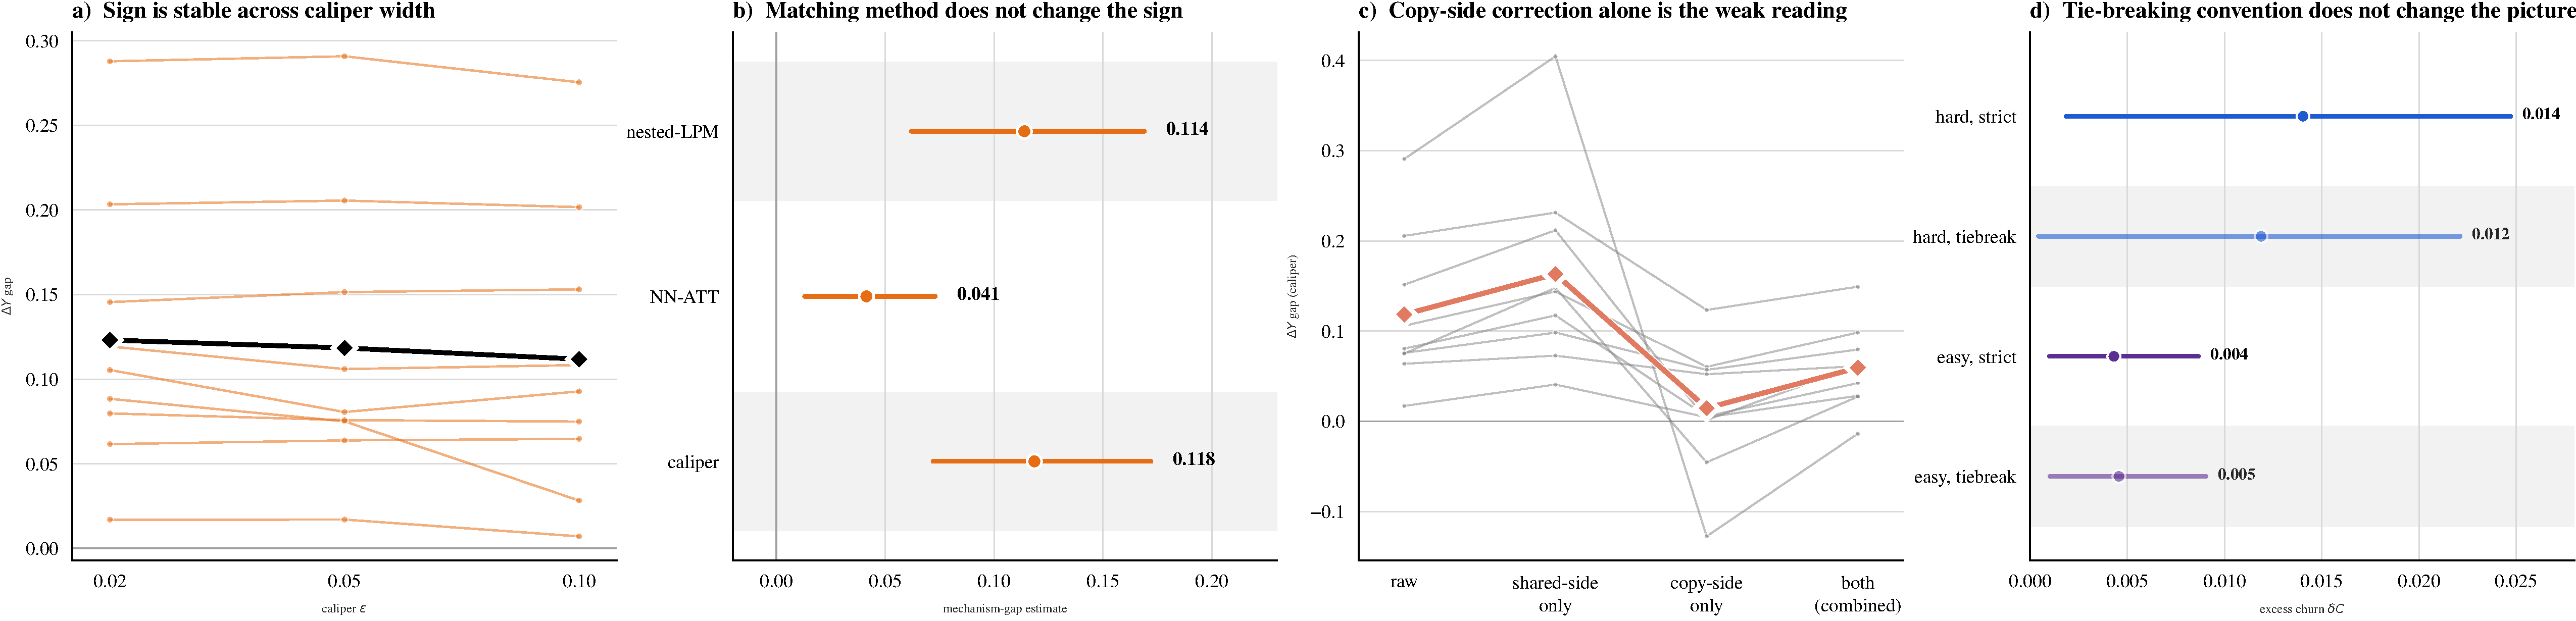
\includegraphics[width=\linewidth]{figures/f5_main_robustness.pdf}
\captionof{figure}{\textbf{Sensitivity to matching and noise correction.} \textbf{(a)} Fourteen specifications ranked by equal-pair mean; grey lines show pairs, whiskers uncorrected macro $95\%$ CIs. \textbf{(b)} Specification settings.}
\label{fig:robustness}
\end{minipage}
\end{center}

\par\addvspace{6pt}

\end{document}
